\chapter{Background and related work}
\label{chap:background}

Knowledge representation (KR) is an area of artificial intelligence research which deals with representing knowledge using  symbols, thus allowing the application of automated reasoning techniques to infer new knowledge from given knowledge \cite{brachman2004aa}. KR forms the basis of \emph{knowledge-based systems}, \enquote{intelligent} systems which make use of a \emph{knowledge base} (KB) that contains told facts about some domain, as well as procedures to reason over these facts and infer implicit knowledge. While there exists a wide range of approaches to implementing knowledge-based systems, such as logic programming \cite{baral94aa}, frames \cite{minsky74aa}, and semantic networks \cite{sowa87st}, in this thesis we are dealing with description logics (DLs) \cite{dlhb03} as the underlying knowledge representation formalism for knowledge bases. DLs are a family of logics based on a guarded fragment of first-order logic which is more expressive than propositional logic, while still being decidable \cite{dlhb03}.

This chapter introduces the basic concepts of description logics, which underpin the Web Ontology Language OWL \cite{horrocks03vn,cuenca-grau08kw}. It outlines the syntax and semantics of description logics and fixes relevant notions such as \emph{axioms} and \emph{entailments} of an OWL ontology. It also discusses the landscape of logical and non-logical errors occurring in OWL ontologies, which motivates the need for tailored debugging support. It then introduces \emph{justifications} as an explanation service for entailments of OWL ontologies, and reviews the literature dealing with justification-based explanation. This covers approaches to computing single and multiple justifications, as well as the issues of understanding justifications, justification-based repair of errors, and coping with multiple justifications, which is the main focus of this thesis.

\section{Description logic knowledge bases}

In the first part of this chapter, we will give an introduction to the basic concepts of description logics, such as the description logic syntax and semantics, and the standard reasoning services used with description logic knowledge bases. We will then discuss the relationship between description logics and the Web Ontology Language OWL, and give a brief overview of the different applications of OWL.

\subsection{DL syntax and semantics}

\subsubsection{DL syntax}

The main building blocks of DLs are atomic \emph{concepts}, \emph{roles}, and \emph{individuals}. With respect to their relationship with first-order logic (FOL), concepts correspond to unary predicates in FOL, roles to binary predicates, and individuals to constants. These entities are used to create more expressive concept and role expressions with the help of constructors, whereby the available constructors depend on the expressivity of the respective DL. As a convention, we will be using the upper-case letters \dlcn{A} and \dlcn{B} for atomic concepts and \dlcn{C}, \dlcn{D}, \ldots for possibly complex concepts; the lower-case letters \dlcn{r}, \dlcn{s}, \ldots for role names, and the lower-case letters \dlcn{a}, \dlcn{b}, \ldots for individuals.

The basic description logic \dl{ALC} (\enquote{Attribute Logic with Complement}) \cite{schmidt-schauss91bc}, which many other more expressive DLs build upon, allows concept expressions as defined by the following grammar:
\begin{align*}
C, D ::= \top \mid \bot \mid A \mid \neg C \mid C \conj D \mid C \disj D \mid \exists r.C \mid \forall r.C
\end{align*}

Given a concept expression $C$, the \emph{modal depth} of the expression is the maximum nesting depth of constructors in $C$. The \emph{length} of an expression is the number of occurrences of concept, role, and individual names, as well as constructors. For example, the expression $A \conj \forall r.(\exists s.(B \conj C))$ has a modal depth of two and a length of nine.
 
\subsubsection{Axioms}

A description logic knowledge base \K is generally regarded as a finite set of axioms which are \emph{asserted} in the KB. Axioms are sentences that make statements about the domain knowledge modelled in the KB. The axioms in a KB are classified into the sets of \emph{TBox}, \emph{RBox} and \emph{ABox} axioms which are denoted as \tbox, \rbox, and \abox, respectively: \K = $\langle \tbox, \rbox, \mathcal{A}\rangle$. The \emph{signature} \sig{\K} of a knowledge base \K is the set of all concept, role, and individual names occurring in \K.

A TBox axiom \axiom is either a \emph{subsumption} (\dlax{C \subcls D}) or \emph{equivalence} (\dlax{C \eqcls D}) between two (possibly complex) concepts \dlcn{C} and \dlcn{D} in a knowledge base. A subsumption axiom expresses that \dlcn{C} is a sub-concept of \dlcn{D}; that is, every instance of \dlcn{C} is also an instance of \dlcn{D}. We can say that \dlcn{C} \enquote{is-a} \dlcn{D}. Equivalence axioms state that two concepts \dlcn{C} and \dlcn{D} are equivalent, which corresponds to (and is a shorter notation for) a bi-directional subsumption \dlax{C \subcls D} and \dlax{D \subcls C}.

Subsumption and equivalence are also possible between roles, which are described by RBox axioms:\footnote{Note that the use of RBox axioms as described here already goes beyond the basic description logic \dl{ALC}.} \dlax{r \subcls s} specifies that \dlcn{r} is a sub-role of \dlcn{s}, which means that every two individuals that have an \dlcn{r}-relationship also have an \dlcn{s}-relationship between them. \dlax{r \eqcls s} expresses that the two roles are equivalent. Further, we can specify axioms containing role \emph{chains} \dlax{r \circ s \subcls t}, which states that if an individual $a$ has an $r$-successor $b$, and $b$ has an s-successor $c$, then it also holds that $a$ has a $t$-relationship with $c$.

ABox axioms make statements about the relations between individuals and concepts, and between individuals and roles: \dlax{C(a)} expresses that the individual \dlcn{a} is an instance of the concept \dlcn{C}, and \dlax{r(a,b)} specifies that there exists an \dlcn{r}-relationship between the individuals \dlcn{a} and \dlcn{b}.

As an example, we use a small knowledge base \K = $\langle \tbox, \mathcal{A}\rangle$ that describes the eating habits of animals on an abstract level:
\begin{examp}
\begin{align*}
		\T = \{&\ax{Cat \sqsubseteq Carnivore}, \ax{Carnivore \sqsubseteq Animal \conj \forall eats.Animal},\\ 
		& \ax{Plant \sqsubseteq \lnot Animal}, \ax{Grass \sqsubseteq Plant} \\ 
		& \ax{PetOwner \equiv Human\conj \exists hasPet.Animal}, \ax{\exists eats.\thing \subcls Animal}\}\\
		\A = \{& \ax{Cat(Molly)},\ax{Human(Alice)},\ax{hasPet(Alice, Molly)}\}\label{ex:petkb}
	\end{align*}
\end{examp}

The TBox of this example KB consists of axioms that make statements about the concepts in the domain: cats are carnivores, a carnivore is an animal which only eats animals, plants are disjoint with animals (i.e.\ no one thing can be a plant and an animal at the same time), grass is a plant, a pet owner is a human who has an animal as a pet, and everything that eats something is an animal. The ABox contains statements about individuals (\cn{Molly} is a \cn{Cat}, \cn{Alice} is a \cn{Human}), and the relationship between them (\cn{Molly} is \cn{Alice}'s pet).

A TBox is called \emph{acyclic} if it does not contain any axioms or chains of axioms where an entity occurs in both the right- and the left-hand side of a subsumption or equivalence. That is, an axiom of the type \dlax{C \subcls \exists r.C} would cause a TBox to be cyclic. Axioms containing only atomic concepts on the left-hand side are called \emph{definitions}, and an \emph{acyclic} TBox containing only definitions where all concepts on the left-hand side have unique names is called a \emph{definitorial} TBox. \emph{General} TBoxes may contain \emph{general concept inclusion} (GCI) axioms, which allow complex concept expressions on both the right- and the left-hand side, such as \ax{\exists eats.\thing \subcls Animal}.


\subsubsection{Naming conventions}

The name of a description logic is generally comprised of mnemonics representing the available constructors and axiom types in the respective logic: the letters \dl{N} and \dl{Q} stand for unqualified (\dlax{\geq n r}, \dlax{\leq n r}) and qualified number restrictions (\dlax{\geq n r.C}, \dlax{\leq n r.C}), respectively (for $n \in \mathbb{N}$, $r$ a role), \dl{F} represents the functionality of roles (\dlax{\geq n r}), \dl{H} stands for role hierarchies (\dlax{r \subcls s}), \dl{I} is the role inverse \dlcn{\inv{r}}, \dl{R} stands for complex role inclusions of the type \dlax{r \rcirc s \subcls r}. The letter \dl{O} denotes the presence of nominals, which allows the use of individuals in the place of concepts in TBox axioms: \dlax{C \subcls \{a\}}. 

Some notable description logics, besides the aforementioned \dl{ALC}, include \dl{S} \cite{horrocks99wq} which corresponds to \dl{ALC+} (\dl{ALC} plus role transitivity), the less expressive \dl{EL} \cite{brandt04ub} which allows existential quantifiers and intersection, \elplusplus \cite{baader05aj} which corresponds to \dl{EL} plus complex role inclusions and nominals, and the highly expressive logics \dld{SHOIN} \cite{horrocks03vn} and \dld{SROIQ} \cite{horrocks06ya} which underpin OWL and OWL 2, respectively. In the context of OWL, the suffix $(D)$ indicates the use of XML Schema\footnote{\url{http://www.w3.org/TR/xmlschema11-2/}} datatypes.


\subsubsection{Model-theoretic semantics}

The semantics of description logics is model-theoretic and given by interpretations. An interpretation \I is a tuple \interpretation, where \deltai is the interpretation domain, that is, a non-empty set of elements, and \doti the interpretation function. The interpretation function maps concept names $A$ in the knowledge base to sets $A\interp \subseteq \deltai$, role names to sets $r\interp \subseteq\deltai \times \deltai$, and individuals to elements in \deltai. We call the set $C\interp$ the \emph{extension} of the concept $C$ in \I. The interpretation function for concepts, roles, and individuals in \dl{ALC} is defined in Table \ref{tab:alcinterp}.

\begin{table}[htb]
\centering
\caption{\dl{ALC} constructors and semantics.}
\begin{tabu}{rll}
\toprule 
Constructor 										& Syntax 					& Semantics \\ 
\midrule
Top concept 									& $\top$ 					& $\deltai$ \\ 
Bottom concept 								& $\bot$ 					& $\emptyset$ \\ 
Concept negation								& $\neg C$				& $\deltai \setminus C\interp$ \\ 
Concept intersection (conjunction) 	& $C \conj D$ 		& $C\interp \cap D\interp$ \\ 
Concept union (disjunction) 			& $C \disj D$ 		& $C\interp \cup D\interp$ \\ 
Existential restriction 						& $\exists R.C$		& $\{ x \mid \exists y . \interp \langle x, y \rangle \in r\interp \wedge y \in C\interp \}$ \\ 
Universal restriction 						& $\forall R.C$ 		& $\{ x \mid \forall y . \interp \langle x, y \rangle \in r\interp \rightarrow y \in C\interp \}$\\ 
\bottomrule
\end{tabu} 
\label{tab:alcinterp}
\end{table}

An interpretation \I is a \emph{model} for an axiom \axiom if it \emph{satisfies} \axiom; we write \I \entails \axiom if \dlax{C\interp \subseteq D\interp} in \I for a subsumption $\alpha = C \subcls D$, and if \dlax{C\interp =  D\interp} in \I for $\alpha$ an equivalence axiom \dlax{C \eqcls D}. A model of a knowledge base \K is an interpretation \I in which \emph{all} axioms in \K are satisfied: \I \entails \K. A \emph{tautology} is an axiom which is always interpreted as \thing; for example, the axiom \dlax{A \subcls A} is a tautology, as $A\interp \subseteq A\interp$ holds in \emph{all} models \I of \K.

\subsection{Standard reasoning services}
The ability to convey information without having to explicitly state it is one of the main advantages of logic-based knowledge bases. A description logic \emph{reasoner} is a piece of software which implements a decision procedure for the standard reasoning problems:

\begin{compactdesc}
\item[Consistency] Given a knowledge base \K, determine whether there exists an interpretation \I for \K such that \I \entails \K. If there exists such an interpretation, return \enquote{true} (the KB is consistent), otherwise return \enquote{false} (the KB is inconsistent). All other reasoning services can be reduced to consistency checking in logics that support conjunction and negation.
\item[Satisfiability]
A concept \dlcn{C} is satisfiable if there is \emph{some} model of \K in which \dlcn{C} is not empty: $C\interp \neq \emptyset$ in some \I that is a model \K. \dlcn{C} is unsatisfiable, denoted as $\K \models C \sqsubseteq \bot$, if it is mapped to the empty set in \emph{all} models \I of the knowledge base.
\item[Subsumption]
One of the main reasoning task in DLs is \emph{subsumption} between concept expressions, i.e.\ checking whether the extension of a (potentially complex) concept $C$ in \K is a subset of the extension of another concept $D$ ($C\interp \subseteq D\interp$). The subsumption between two concepts where $C$ is necessarily interpreted as a subset of $D$ is denoted as $\K \models C \sqsubseteq D$.
\item[Equivalence] 
Two concepts $C$ and $D$ are \emph{equivalent} in the KB ($C \equiv D$), if it holds that all elements of $C\interp$ are in the set $D\interp$ and vice versa, i.e.\ if $C\interp = D\interp$, in all models \I of \K. Equivalence is a special case of subsumption.
\item[Instantiation]
Instantiation (or instance checking) checks which individuals are instances of a particular concept: given an individual \dlcn{a}, a concept \dlcn{C}, and a KB \K, return \enquote{true} if \dlcn{a\interp}  $\in$ \dlcn{C\interp} in all models \I of \K.

\end{compactdesc}

There exist a number of sound, complete, and terminating algorithms for providing the above reasoning services, which are implemented by  description logic reasoners: \emph{Tableaux} \cite{de-giacomo96ez,horrocks97cf,horrocks00dy,baader00va} procedures attempt to build a finite tree-like model of the concepts in the knowledge base using \emph{tableau rules}. The input is first translated into negation normal form (NNF) and then decomposed according to the respective tableau rules. The nodes and edges in the tree are labelled with the decomposed concepts and roles, respectively. A \emph{clash} in the tree occurs when the algorithm attempts to label a node in the tree with contradictory concepts, such as an atomic concept $A$ and its negation $\neg A$.

When no more rules are applicable to the concept fragments, or when a clash occurs, the algorithm terminates. If some clash-free tree (i.e.\ some model) can be found for a concept \dlcn{C}, the concept is satisfiable. Likewise, if no clash-free tree can be found, the concept has no models, i.e.\ it is unsatisfiable. The types and usage of constructors in a description logic affect the types of rules used in a tableau algorithm, which in turn can increase the computational complexity of the reasoning algorithm. For instance, as some of the tableau rules are non-deterministic (i.e.\ involve choice), the algorithm has to perform backtracking if such a rule has been applied. 


\subsubsection{Entailments}

An entailment \ent of a knowledge base \K is an axiom that follows logically from \K. \K entails \ent (\K \entails \ent) if \ent is true in \emph{all} models \I of \K. The entailment relation is \emph{monotonic} in DLs, which means that entailments are preserved when further axioms are added to the KB. Every axiom which is asserted in \K is an entailment of the knowledge base, while there are other entailments which represent \emph{implicit} knowledge in the KB. For example, the pet KB above explicitly asserts that \ax{Cat \subcls Carnivore} and \ax{Carnivore \subcls Animal \conj \forall eats.Animal}. From these statements we can conclude that every \cn{Cat} is an \cn{Animal}: \K \entails \ax{Cat \subcls Animal}. 

Entailments are not restricted to any specific axiom type; for example, the axioms \ax{Cat \subcls Carnivore} and \ax{Carnivore \subcls Animal \conj \forall eats.Animal} also entail the statement \ax{Cat \sqsubseteq \forall eats.Animal}. The set of all axioms which are valid in a description logic \L and entailed by a KB \K is called the \emph{deductive closure} of \K:

\begin{defn}[Deductive closure]
The deductive closure \closure{\K_{\L}} of a knowledge base \K is the set of \L-axioms entailed by \K, i.e.\  $\closure{\K_{\L}} = \{ \alpha \in \L \mid \K \models \alpha \}$. When clear from the context, the subscript \L is dropped.
\end{defn}

Even KBs based on weakly expressive DLs have infinitely many entailments (i.e.\ the deductive closure is infinite). The simplest example is the \emph{empty} knowledge base \K over a non-empty signature \sig{\K} = \{$A$\} in the logic \dl{ALC}. The deductive closure of \K then is the infinite set of all axioms that can be formed using $A$ and the available constructors in \dl{ALC}:
\begin{align*}
\closure{\K} = \{ A \subcls A, A \conj A \subcls A, A \disj A \subcls A, A \subcls A \conj \thing, \ldots \}
\end{align*}

The focus when constructing and analysing a knowledge base often lies on the \emph{concept hierarchy} of the KB, which is represented by its entailed atomic subsumption axioms. In the context of this thesis, we simply speak of an \emph{entailment set} to denote a \emph{finite} set of entailments of a knowledge base \K, restricted by some clearly specified criteria:
\begin{defn}[Entailment set]
An entailment set \entsetk of a knowledge base \K is a finite set of axioms $\{ \alpha_{i} \mid i \in \{1 .. n \} \} \subseteq \closure{\K}$.
\end{defn}

An in-depth discussion of the issue of specifying useful finite entailment sets follows in Chapter \ref{chap:entailments}.

\subsubsection{Incoherence}
A concept $C$ is \emph{unsatisfiable} in a knowledge base \K if there is no model \I of \K in which $C\interp$ is non-empty. This means that the concept cannot have any instances. Unsatisfiability is caused by contradictory statements, such as \dlax{C \subcls D \conj \neg D}. A KB that contains some unsatisfiable named concept is called \emph{incoherent}. 

Continuing with the previous example KB, we can induce incoherence in \K' = $\langle \tbox', \mathcal{A}\rangle$  by adding the last TBox axiom which causes the concept \cn{SickCat} to be  unsatisfiable:
\begin{examp}
\begin{align*}
		\T' = \{&\ax{Cat \sqsubseteq Carnivore}, \ax{Carnivore \sqsubseteq Animal \conj \forall eats.Animal},\\ 
		& \ax{Plant \sqsubseteq \lnot Animal}, \ax{Grass \sqsubseteq Plant} \\ 
		& \ax{PetOwner \equiv Human\conj \exists hasPet.Animal}, \ax{\exists eats.\thing \subcls Animal}, \\
		& \ax{SickCat \eqcls Cat \conj \exists eats.Grass}\}\\
		\A = \{& \ax{Cat(Molly)},\ax{Human(Alice)},\ax{hasPet(Alice, Molly)}\}
	\end{align*}
\end{examp}
The conflict is caused by the TBox axioms in \K' which entail that \cn{Cats} are \cn{Carnivores}, thus eating only \cn{Animals}, but that instances of \cn{SickCat} eat \cn{Grass}, a concept which is a subconcept of \cn{Plant}, thus known to be disjoint with \cn{Animal}.  As, according to our knowledge base, there cannot exist a \cn{Carnivore} who also eats \cn{Grass}, the concept \cn{SickCat} cannot have any elements in any model \I of \K': $SickCat\interp = \emptyset$. Therefore, the concept \cn{SickCat} is said to be unsatisfiable, and the knowledge base \K' is incoherent.

\subsubsection{Inconsistency}
While incoherence itself does not cause any reasoner problems (as the concept simply corresponds to the empty set in all models), instantiation of unsatisfiable concepts causes the KB to be contradictory. If the axiom \cn{SickCat(Molly)} is added to the KB in which \cn{SickCat} is unsatisfiable, it is not possible for the KB to have any model in which this statement is satisfied. Such a knowledge base that has no models is called \emph{inconsistent}, which is denoted as \K $\models \top \sqsubseteq \bot$. 

An inconsistent KB has the property that it entails \emph{everything} that can be expressed in the respective logic \L---since it is contradictory, it cannot possibly make any meaningful statements about the knowledge it models. Different approaches to reasoning with inconsistent knowledge bases have been explored, such as \emph{paraconsistent} reasoning \cite{ma07yl}, or the selection of a consistent subset based on a relevance function \cite{huang05du}. 


\subsection{The Web Ontology Language OWL}


\subsubsection{From description logic to OWL}

While \enquote{ontology} is a term borrowed from philosophy, in computer science it describes a software artefact representing information about the entities in a domain, and the relationships between them \cite{gruber93xg}. In the remainder of this thesis, we will use the term \emph{ontology} (denoted by the letter \O) to refer to a description logic knowledge base which is represented in some machine-processable format, such as OWL. 

OWL is a successor of the web ontology language DAML+OIL \cite{horrocks02aa}, a description logic based ontology language with an RDF/XML syntax which evolved from merging DAML-ONT (a language developed by the DARPA Agent Markup Language programme) and OIL (Ontology Inference Layer, developed by the European \emph{On-To-Knowledge} project). The first version of OWL, which is based on the expressive description logic \dld{SHOIN} and was described as a \enquote{revision} of DAML+OIL, became an official W3C recommendation in February 2004.\footnote{\url{http://www.w3.org/TR/owl-features/}} 

OWL may also be regarded as a more expressive successor to RDF (Resource Description Framework) \cite{w3c04aa}, a language to describe relationships between entities using subject-predicate-object style \emph{triples}, and RDFS (RDF Schema) \cite{w3c04ab}, an extension of the RDF vocabulary which introduces \enquote{meaningful} predicates such as \texttt{Class}, \texttt{subClassOf}, and \texttt{domain}.

OWL 2, the successor of OWL, was made a W3C recommendation in 2009 \cite{w3c09eu}. It comprises two species of different expressivities, namely OWL 2 DL and OWL 2 Full. The underlying formalism of OWL 2 DL is the description logic \dld{SROIQ} \cite{horrocks06ya}. This highly expressive DL adds a range of constructors and axiom types to those of \dl{ALC}, such as complex role inclusions (represented by the letter \R), nominals (\O), inverse roles (\I), qualified number restrictions (\Q), and datatypes ($D$). While OWL 2 DL has the familiar description logic semantics (\emph{Direct Semantics}) described above, OWL 2 Full \cite{w3c12aa} has an RDF-based semantics, which is a superset of the OWL 2 Direct Semantics.

There exist several syntaxes for OWL \cite{horridge10aa}, such as the human-oriented Manchester Syntax \cite{horridge06aa}, various RDF formats, and an OWL/XML serialisation. The axiom \ax{Carnivore \sqsubseteq Animal \conj \forall eats.Animal} from the above example is written as follows in OWL Manchester Syntax (keywords are set in italics):
\begin{flalign*}
&\mathit{Class\!:} ~ \mathsf{Carnivore} & \\
&\;\;\;\mathit{SubClassOf\!:} ~ \mathsf{Animal} ~\mathit{and} ~ \mathsf{eats} ~ \mathit{only} ~ \mathsf{Animal} &
\end{flalign*}

In addition to the different syntaxes, OWL also introduces corresponding terms for the entities used in ontologies: \emph{concepts} are referred to as \emph{classes}, \emph{roles} become \emph{properties}, the top concept \thing is referred to as \cn{Thing}, and the bottom concept \nothing as \cn{Nothing}. For the remainder of this thesis, we will switch to using OWL lingo to refer to classes, properties, (sub-)expressions, and ontologies. Further, in the context of this thesis we will simply regard OWL 2 DL as a syntactic variant of \dl{SROIQ}, using the name OWL in place of OWL 2 DL, unless otherwise stated. 

\subsubsection{Usage of OWL}

OWL was designed with the aim of providing an expressive machine-processable ontology language for use in various applications and domains. There exists a wide array of tools and libraries for creating and editing OWL ontologies, such as \protege,\footnote{\url{http://protege.stanford.edu/}} \tbc,\footnote{\url{http://www.topquadrant.com/products/TB\_Composer.html}} \swoop,\footnote{\url{https://code.google.com/p/swoop/}} the OWL API,\footnote{\url{http://owlapi.sourceforge.net/}} a Java library that gives access to a large number of ontology editing tasks and reasoner interfaces, a number of highly optimised OWL reasoners, such as Pellet \cite{sirin07ws}, HermiT \cite{shearer08td}, and FaCT++ \cite{tsarkov06np}, as well as reasoners which are tuned towards specific subsets of OWL, such as \emph{ELK} \cite{kazakov11aa}, a reasoner for \elplusplus ontologies. 

This broad set of OWL tools allows users to choose a suitable development environment for their respective application requirements, and improved tool support is being regarded as one of the main reasons for the growing use of OWL ontologies as a knowledge representation mechanism \cite{horridge08yi}.


\paragraph{OWL 2 profiles}

There exist three named \enquote{profiles} for OWL 2, syntactic subsets of OWL 2 DL that are tailored towards different applications, which trade expressivity of the language for efficient reasoning:

The OWL 2 EL profile is a tractable fragment of OWL 2 which is based on the description logic \elplusplus \cite{baader05aj}. OWL 2 EL omits some of the more expressive OWL 2 constructors in favour of efficient reasoning (polynomial time), which makes it attractive for use in ontologies that \enquote{contain very large numbers of properties and/or classes} \cite{owl2profiles2009}.

OWL 2 QL (Query Language), which is based on the \emph{DL-Lite} family of description logics \cite{artale2009aa}, has been defined for use in applications which focus on query answering over large amounts of instance data. The queries executed against OWL 2 QL ontologies can be rewritten into SQL queries, which allows storing instance data in a standard relational database, thus significantly improving query performance. OWL 2 QL is used for ontologies in  Ontology-Based Data Access (OBDA) systems, which combine OWL 2 QL reasoning with efficient querying over relational databases \cite{calvanese2011aa,rodriguez-muro2012aa}.

Reasoning systems for ontologies in the OWL 2 RL (Rule Language) profile can be implemented using rule-based reasoning engines. Similar to OWL 2 QL, the profile restricts the use of constructors to certain positions in axioms, e.g.\ universal restrictions and negation are only allowed on the RHS of axioms. While OWL 2 RL allows the use of a wider range of expressive constructors than the other two OWL 2 profiles, these positional restrictions lead to efficient reasoning performance.

\paragraph{Semantic Web} The idea of a Semantic Web \cite{berners-lee01bf} marks a move away from a human-oriented  \enquote{web of documents} towards a machine-oriented \enquote{web of data}. By enriching web pages with semantic content we can express relationships between entities on the web, thus allowing understanding of those relationships by automated processes rather than direct human processing. This \enquote{meaningful} interlinking of web content is thought to improve searching for and integrating information on the web. 

As a \enquote{source of shared, precisely defined terms} \cite{horrocks02aa}, ontologies play a key role in the Semantic Web,  with the majority of ontologies found on the web using OWL or RDF(S) \cite{cardoso07xj}. Examples of prominent OWL ontologies on the web include the BBC Programmes and Wildlife ontologies,\footnote{\url{http://www.bbc.co.uk/ontologies/}} and the set of geographical ontologies created by Ordnance Survey.\footnote{\url{http://www.ordnancesurvey.co.uk/oswebsite/ontology/}} However, while OWL has been designed specifically as an ontology language for the Semantic Web, its \emph{perceived} complexity and unpredictable reasoning performance still prohibit wider uptake by web application developers, for whom \enquote{a little semantics} \cite{hendler07aa} in the form of RDF may often seem sufficient.

\paragraph{Medical informatics and life sciences}
OWL ontologies are frequently used for the encoding of biological and medical knowledge as part of larger information systems. Examples for intensively used and maintained medical OWL ontologies include the SNOMED CT ontology\footnote{\url{http://www.ihtsdo.org/snomed-ct/}} which contains medical terminology used in electronic health records, the OWL version of the International Classification of Diseases (ICD-10) catalogue\footnote{\url{http://www.who.int/classifications/icd/en/}} released by the World Health Organization (WHO), and the National Cancer Institute (NCI) thesaurus\footnote{\url{http://ncit.nci.nih.gov/}} which covers knowledge related to cancer, such as anatomy, findings, drugs, and genes. 

There exists a vast array of biological ontologies of varying size and expressivity, such as the Gene Ontology, which aims to \enquote{standardize the representation of gene and gene product attributes}, the Experimental Factor Ontology (EFO) which models variables in biological experiments, and various ontologies describing the anatomy of species. Finally, the NCBO BioPortal \cite{noy09jc} is a prominent curated collection of biomedical ontologies that were created by a number of research groups which has received some attention in recent years as a popular test corpus for OWL ontology research \cite{bail11jm,horridge11ac,horridge12aa,mikroyannidi12qf}.


%%%%%%%%%%%%%%%%%%%%%%%%%%%%%%%%%%%%%%%%%%%%%%%%%%%%%%%%%%%%%%%%%%%%%%%


\section{Errors in OWL ontologies}

OWL is a highly expressive ontology language which offers users a wide range of constructors for modelling domain knowledge at a high level of precision. The downside of this expressivity is that constructors can be misinterpreted by users, and combinations of otherwise correct axioms may lead to undesired side-effects. Beyond side-effects caused by human users, common engineering tasks such as translation of an ontology into OWL from some other formalism, automated generation of an ontology using some input source, or integration of an existing ontology, may also introduce errors into an ontology.

We mainly distinguish between two different types of errors: \emph{logical errors}, which can be detected through the use of a reasoner, and \emph{non-logical errors}, which range over incorrect statements with respect to the domain knowledge modelled in the ontology, modelling inconsistency, reasoner performance issues, and annotation problems. In this section, we will give an overview of the different errors users may encounter in the OWL ontology development process, and describe how these errors are commonly detected and repaired.

\subsection{Logical errors}

\subsubsection{Unsatisfiable and tautological classes}
A common logical error is the unsatisfiability of a named class \emph{A} in an ontology \O, which implies that \emph{A} cannot have any instances. While the unsatisfiability of a class \emph{may} be intentional (e.g.\ for testing purposes as suggested by the \protege OWL tutorial \cite{horridge11aa}, to explicitly prohibit a certain definition for a class, or to introduce a new name for \nothing), it mostly indicates a modelling error caused by contradictory statements. Unsatisfiable classes are easily detected by a reasoner and are commonly highlighted as errors in OWL editing tools, for example by rendering them in red colour, or by arranging them as a subclass of \nothing.

Likewise, we call a class \dlcn{B} in an ontology \O \emph{tautological} if \O entails that \dlax{\thing \eqcls B}, that is, every class in the domain is entailed to be a subclass of \dlcn{B}, and every individual is entailed to be an instance of \dlcn{B}. As with unsatisfiable classes, a tautological class may be introduced on purpose to achieve that very same effect. However, we know that tautological classes often occur accidentally and without ontology users noticing or understanding why something is entailed to be equivalent to \thing \cite{horridge09ct}. This phenomenon may also cause unwanted side effects, such as the unsatisfiability of a class that is asserted to be disjoint with the tautological class, as we have seen in the \emph{Movie} ontology example \cite{horridge09ct}, which we will describe in Section \ref{sec:justproofs}. While tautological classes can also be detected by a reasoner, they are generally not treated as errors in OWL tools.


\subsubsection{Inconsistency}
By instantiating an unsatisfiable class, i.e.\ specifying that an individual is an instance of an unsatisfiable class, an ontology becomes \emph{inconsistent}, or \emph{contradictory}. Inconsistency can also be caused by a TBox which contains axioms that prohibit any class from having a non-empty extension, for example by using an axiom of the type \dlax{A \disj \neg A \subcls B \conj \neg B}. Inconsistency is a severe logical error as it causes the ontology to entail \emph{every} axiom, which makes it impossible (under standard semantics) to infer meaningful information from the ontology; this renders the ontology useless. In order to prevent the inconsistency of an ontology, it is highly desirable to \emph{repair} any unsatisfiable classes as soon as they arise in the ontology engineering process.


\subsubsection{Wrong entailments}

Some logical errors, such as incoherence and inconsistency, can be detected using a reasoner, as detection is simply reduced to entailment. Factual errors (wrong and unwanted entailments), however, can only be spotted by a user with the appropriate domain knowledge.

While there may be some knowledge in the world which we can consider facts (such as \enquote{the parent of every human is a human}---for the time being, there is little to argue about this statement), we often come across knowledge and relationships which are and \emph{cannot} be clearly defined. Thus, we can say that every ontology is subject to an \emph{ontological commitment} which prescribes relations in the ontology depending on the \emph{view} we have on a domain. Going back to the parent--human relationship, what happens if we build a knowledge base that is a representation of creatures from Greek mythology? In such an ontology we can imagine the need to allow a human to have a non-human parent; yet, given our restriction that humans have only human parents, this would be impossible. 

While mythological creatures may be a very specific example, we can quickly see cases in which such a restriction can lead to more fundamental debates. A frequently occurring issue is that of gender: general knowledge tells us that there are two genders, and every person \emph{has} to be either male or female (but not both), which we may model as such in an ontology. And yet, this is clearly an issue which ranges far beyond knowledge modelling techniques, as the gender binary has long been the focus of fundamental biological and political debate. When talking about \emph{errors} in an ontology, we have to bear in mind that some errors may not be statements which are intrinsically wrong, but simply \emph{wrong in the context of the ontology.}

Besides factual errors caused by ambiguities and the difficulty of modelling certain aspects of a domain, wrong entailments can also stem from incorrect use of OWL constructors. We have a good understanding of the common errors that users make when constructing OWL ontologies \cite{rector04aa,kalyanpur06bh,roussey09ab}. Some of these errors include confusing \enquote{and} and \enquote{or}, subsumptions and equivalences, \enquote{forgetting} previously defined property restrictions, and introducing axioms which do not have any effect on the model of the ontology. Given a catalogue of such \emph{antipatterns}, an OWL tool can point out axioms that are potentially erroneous and provide further explanation of the semantics to a user. Kalyanpur et al.\ \cite{kalyanpur06bh} use a set of common modelling errors in a heuristics-based repair tool in the \swoop ontology editor which suggests removal or modification of axioms based on, amongst other aspects, the likelihood of them being incorrect.

\subsubsection{Non-entailments} 

Missing entailments, or non-entailments, are frequently occurring errors in OWL ontologies which are particularly hard to detect. When constructing an ontology, developers expect certain entailments, such as an obvious subsumption between two classes, to be caused by the axioms they add; if an expected (and desired) entailment does not follow from the ontology, this may be considered an error. Roussey et al.\ \cite{roussey09ab} found that ontology developers frequently add axioms to ontology that either do not have the desired effect, or no effect at all. In these cases, \emph{ontology diff} tools (e.g.\ \cite{franconi10bg,goncalves11xz,kremen11yc}) can help users spot whether any modifications to an ontology had the desired effect; beyond the detection of ineffectual modifications, however, dealing with non-entailments is a non-trivial task.

A structured approach to eliciting missing entailments and adding them to the ontology is \emph{ontology completion} \cite{baader07aa}, which is based on methods from the area of Formal Concept Analysis (FCA) \cite{ganter05ar}. An ontology completion tool presents users with a series of potential entailments, e.g.\ a subsumption between two classes, asking them to accept or reject the presented entailment. In case of an accepted entailment, an axiom is added to the ontology to explicitly state the relationship; otherwise, the tool asks the user to produce a \emph{counter-example} to ensure that the axiom is not entailed. 

If we look at non-entailments from a different angle, the non-entailment of a \emph{negative} entailment may also be considered an error. OWL is based on the \emph{Open World Assumption} which means that anything that is not explicitly forbidden is considered to be a \enquote{don't know} rather than a \enquote{no}. For instance, in the above example ontology we did not explicitly state that \cn{Human} and \cn{Cat} are disjoint classes; that is, at a later point, we could add the statement \cn{Human(Molly)} to the existing \cn{Cat(Molly)} without causing a logical error in the ontology. While the error then falls into the category of unwanted entailments, it may be useful to \emph{prevent} such problems before they even occur. Similar to ontology completion, \emph{semantic clarification} \cite{schlobach05tf} aims to prevent unwanted entailments by strengthening the ontology with disjointness axioms where appropriate.


\subsection{Non-logical errors}


\subsubsection{Structural irregularities}
There exists a number of ontology design patterns \cite{gangemi05cr,aranguren08nx} which provide  solutions for situations that are difficult to model in OWL, such as representing n-ary relations. But even without such formal patterns, ontologies often exhibit syntactic regularities due to habits or training of ontology engineers \cite{mikroyannidi12qf}. Such regularities include \enquote{good practice} strategies such as adding domain and range axioms for every newly introduced object property. When a specific design pattern or design style is chosen for an ontology, it should be adhered to across the ontology in order to maintain a uniform modelling style. Therefore, deviating from a given structure and existing regularities may be considered an error in the ontology. Ontology pattern inspection tools, such as the RIO \protege plugin \cite{mikroyannidi12aa}, can assist ontology developers in detecting regularities and deviations in OWL ontologies.


\subsubsection{Annotation errors}
Annotations in OWL ontologies are frequently used to convey information about an entity and its relations beyond the logical content of the ontology. One such example is the NCI Thesaurus, in which on average (across a set of 86 subsequent versions of the ontology) over 84\% of the axioms  are annotations \cite{goncalves11as}. It is possible for an annotation to be erroneous, for example, by containing false or missing information about the entity it annotates. Other than manual inspection (or specifically tailored text processing of the annotation strings), there is no way to detect an incorrect annotation.

\subsubsection{Performance problems}
The performance of reasoners for tasks such as classification and query answering over OWL ontologies is one of the main focus points of OWL research. As with \enquote{regular} software, the general user acceptance and usefulness in a production environment of OWL depends, amongst other reasons, on its efficiency.

However, OWL ontologies often turn out to be rather unstable in terms of their performance; even minor changes can seemingly randomly lead from short classification times in the range of seconds to impractical times. Tools which detect  \emph{performance hot spots} \cite{lin08xi,goncalves12uq} can assist ontology developers in identifying ontology subsets which cause a steep increase in classification times. Based upon the hot spot information provided by such a tool, the ontology developer can then remove or rewrite the hotspot-axioms in order to improve the reasoner performance. 

\subsection{Debugging ontologies}

In the context of OWL ontology engineering, the debugging stage involves the process of \emph{detecting} an error in an ontology (e.g.\ an unsatisfiable class, or an incorrect entailment), finding the \emph{source} of the error, i.e.\ the information stated in the ontology which causes the error, and finally, \emph{repairing} the ontology by modifying or removing (some of) the problematic information. Losing as little \emph{correct} information as possible in the repair stage is a key aspect of successful debugging.

In the case of logical errors, the repair process can be performed manually, using a reasoner as a tool to classify the ontology, then searching the class hierarchy for unwanted entailments (potentially aided by a suitable visualisation in an ontology editor, such as \protege which arranges all unsatisfiable classes under the class \cn{Nothing}), tracing the source of the error by inspecting related statements in the ontology, and then modifying those statements that are considered to be incorrect. 

Due to the potential size and complexity of OWL ontologies, this manual approach quickly leads to a tedious process of searching through the entire ontology. Moreover, it may lead to non-optimal repairs, where more information than required is removed or modified for the purpose of fixing the entailment. Anecdotes of ontology developers \enquote{ripping out} parts of the ontology in order to remove an entailment show that this approach is far from ideal and indicates a clear need for additional debugging support.

One of the first approaches to explaining subsumption in description logic ontologies was introduced by McGuinness \cite{mcguinness96rp} and Borgida \cite{mcguinness95jb}, using proof-style explanations for entailments of the CLASSIC knowledge representation system \cite{patel-schneider91tc}. This proof-based approach was later extended by Borgida \cite{borgida99cn} to ontologies in the description logic \dl{ALC}. One of the earliest implementations of debugging facilities in an OWL ontology editor is the explanation component \emph{MEX} in the OntoTrack editor \cite{liebig04lx,liebig05jm}. \emph{MEX} presents natural language proof-style explanations which are based on a tableaux trace as proposed by Borgida et al.\ \cite{borgida99cn} and later extended from \dl{ALC} to cover nearly the complete OWL Lite sub-language of OWL 1 \cite{liebig05jm}. In line with these proof-based approaches, Deng et al.\ proposed a resolution based explanation framework \cite{deng05aa} which was restricted to unsatisfiability and inconsistency of \dl{ALC} ontologies. 

However, it was not until the introduction of \emph{MUPS} (Minimal Unsatisfiability Preserving Sub-TBoxes) \cite{schlobach03nc}, later named \emph{justifications}, that explanation support for description logic ontologies became a key aspect of OWL ontology research, spawning a substantial body of work and several ontology debugging tools.



%%%%%%%%%%%%%%%%%%%%%%%%%%%%%%%%%%%%%%%%%%%%%%%%%%%%%%%%%%%%%%%%%%%%%%%


\section{Justifications for entailments of ontologies}

\emph{Justifications} are the most prominent form of debugging support for entailments of OWL ontologies. They are based on a work by Schlobach and Cornet \cite{schlobach03nc,schlobach07aa}, who developed a strategy for \emph{pinpointing} the causes of unsatisfiable classes in the medical ontology \emph{DICE}.  A justification \J for an entailment \ent of an ontology \O is a minimal subset of \O which is sufficient for \ent to hold:
\begin{defn}[Justification]
\just is a justification for $ \ont \entails \ent$  if $\just \subseteq \ont,  \just \entails \ent$ and, for all $\just' \subset \just$, it holds that $ \just' \nvDash \ent $.
\end{defn}

A justification \justeta is defined with respect to a single entailment \ent; in order to describe the set of \emph{all} justifications for a single entailment, or for the justifications for all entailments in an entailment set \entset, we introduce the notion of \emph{justification sets}:
\begin{defn}[Justification set]
Given an ontology \ont and an entailment $\eta$, the justification set \justseta is the set of all justifications \{$\just_{1} \ldots \just_{n}$\}, $\just_{i} \subseteq \O$, for $\eta$. Likewise, the justification set \justs of an entailment set \entset is the set of all justifications $\J_{i}$ for all $\eta_{k} \in \entset$.
\end{defn}

While Schlobach and Cornet focused on \emph{MUPS} and Minimal Incoherence-Preserving Sub-TBoxes (\emph{MIPS}), that is, minimal entailing subsets for \emph{some} cause of incoherence in \O) in unfoldable \dl{ALC} TBoxes, the concept of explanations based on minimal entailing subsets is applicable to arbitrary entailments. Kalyanpur et al.\ \cite{kalyanpur05mi} extended the idea of \emph{MUPS} to unsatisfiable classes in general OWL ontologies, presenting users with the \emph{sets of support} (which were later named \emph{justifications}, a term borrowed from belief revision  \cite{gardenfors88aa,nebel90dh}) for an entailment. Beyond its application for OWL ontology debugging, computing minimal unsatisfiable cores is also a technique for generating proofs in the SAT community \cite{lynce04fq}.

The minimality of \J implies that removing any one of its axioms \emph{breaks} the entailment \ent. For any entailment \ent of \O, \ent itself is a justification if \ent is asserted in \O, and there can be multiple justifications (exponentially many \cite{baader07xp}) for a single entailment. 

Recall our example from the animal domain which entails that the class \cn{SickCat} is  unsatisfiable:
\begin{examp}
\begin{align*}
		\T' = \{&\ax{Cat \sqsubseteq Carnivore}, \ax{Carnivore \sqsubseteq Animal \conj \forall eats.Animal},\\ 
		& \ax{Plant \sqsubseteq \lnot Animal}, \ax{Grass \sqsubseteq Plant} \\ 
		& \ax{PetOwner \equiv Human\conj \exists hasPet.Animal}, \ax{\exists eats.\thing \subcls Animal}, \\
		& \ax{SickCat \eqcls Cat \conj \exists eats.Grass}\}\\
		\A = \{& \ax{Cat(Molly)},\ax{Human(Alice)},\ax{hasPet(Alice, Molly)}\}
	\end{align*}
\end{examp}
The following axiom set is a justification for \ax{\K' \models SickCat \subcls \nothing}: 
\begin{align*}
\J = & \{ \ax{Cat \sqsubseteq Carnivore},\ax{Carnivore \sqsubseteq Animal \conj \forall eats.Animal}, \\
&\ax{SickCat \equiv Cat \conj \exists eats.Grass}, \ax{Grass \sqsubseteq Plant}, \\
&\ax{Plant \sqsubseteq \lnot Animal} \} \models \ax{SickCat \subcls \nothing}
\end{align*}
In addition to limiting the number of axioms a user has to analyse when presented with a justification, OWL ontology editors generally \emph{order} and \emph{indent} the axioms in justifications, which significantly increases readability. Figure \ref{fig:prot-just-screenshot} shows the above justification as displayed in \protege with ordered and indented axioms.
\begin{figure}
\centering{
	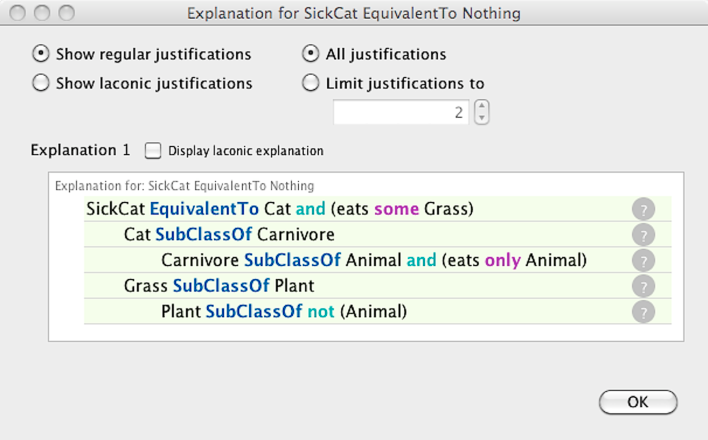
\includegraphics[scale=1]{img/explanation-cat.pdf}
	\caption{A screenshot of the \emph{Explanation} tab in \protege.}
	\label{fig:prot-just-screenshot}
}
\end{figure}

The concept of justifications for description logic ontologies has been widely studied over the past decade, with particular focus on developing efficient algorithms for the computations of all justifications for a given entailment, e.g.\ \cite{schlobach05vd,suntisrivaraporn08aa,du09bn}. There also exist a number of debugging approaches that are closely related to justifications, such as the computation of maximally satisfiable terminologies (MSSs) \cite{meyer06rj,meyer06aa}, which is based on a tableau-like procedure, and the \emph{pinpointing formula} approach proposed by Baader and Pe\~{n}aloza \cite{baader07ur,baader08tp,ji08en,penaloza10ff}.

Rather than directly computing the set of all justifications for an entailment, a pinpointing formula is a compact representation of the set of all justifications for an entailment \cite{baader07ur,baader08tp,penaloza10ff}. A pinpointing formula is a monotone Boolean formula where each propositional variable represents an axiom in the ontology. The set of justifications for an entailment can then be derived from the pinpointing formula as it corresponds to all valuations of the formula. An example of a pinpointing formula is given in \cite{baader07ur}:
\begin{examp}
\begin{alignat*}{2}
 (\alpha_{1})  & \quad\quad & &\dlax{A \subcls \exists r.A}  \\
 (\alpha_{2})  & \quad\quad & &\dlax{A \subcls Y}  \\	
 (\alpha_{2})  & \quad\quad & &\dlax{\exists r.Y \subcls  B}  \\
 (\alpha_{4})  & \quad\quad & &\dlax{Y \subcls B}
\end{alignat*}
\end{examp}
The four axioms labelled with $\alpha_{1}$ to $\alpha_{4}$ entail \dlax{A \subcls B}. We can find two justifications for this entailment: $\J_{1} = \{\alpha_{2}, \alpha_{4} \}$ and $\J_{2} = \{\alpha_{1}, \alpha_{2}, \alpha_{3} \}$. If we treat the axiom labels as propositional variables, the two justifications correspond to the \enquote{true} valuations of the pinpointing formula $\alpha_{2} \wedge ( \alpha_{4} \vee (\alpha_{1} \wedge \alpha_{3} ))$. 

\subsection{Computing justifications}
There exist various approaches to directly computing \emph{one} or \emph{all} justifications for a given entailment, with \enquote{find all} algorithms generally using a \enquote{find one} algorithm as a subroutine. We categorise these algorithms into \emph{glass-box} and \emph{black-box} approaches \cite{kalyanpur05mi}: glass-box techniques generally rely on information provided by a DL reasoner, which requires modification of reasoner internals in order to utilise it for justification computation. By contrast, black-box techniques only use a reasoner as an \emph{oracle} to perform entailment checks.

\subsubsection{Glass-box techniques}

Glass-box justification finding techniques generally rely on the modification of a description logic reasoner to keep track of the axioms required for an entailment to hold, such as those axioms causing a \emph{clash} in a tableaux procedure. More precisely, as the problem of explaining arbitrary entailments, e.g.\ subsumption between classes, can be reduced to a consistency check, this technique can be applied to find justifications for both unsatisfiable classes as well as arbitrary entailments. The tracking strategy applied in glass-box approaches using tableaux reasoners is known as \emph{tracing} \cite{kalyanpur05mi}, which is based on an algorithm first proposed by Baader and Hollunder \cite{baader95aa}. Beyond tableaux-based reasoners, approaches extending the \elplusplus subsumption algorithm \cite{baader07xp} and automata-based approaches \cite{baader08eb,baader10jc} also fall under the label of \enquote{glass box} justification generation. A fair number of approaches to explaining entailments of description logic KBs uses glass-box techniques to present users with reasoner traces in the form of axiom sets, natural language, or some form of visualisation \cite{schlobach03nc,liebig05lf,kwong05aa,meyer06rj}.


\subsubsection{Black-box techniques}

\paragraph{Expand-contract approach}
A simple technique for finding \emph{one} justification for an entailment \ent of an ontology \O is the expand-contract approach \cite{kalyanpur07oq}: in the \emph{expansion phase}, axioms from the given ontology \O are incrementally added to an empty ontology \oprime, performing an entailment check after each addition until it is found that \oprime entails \ent. In order to generate a minimal justification from \oprime, the \emph{contraction phase} then removes superfluous axioms from \oprime, performing an entailment check after each removal. This approach is known as \emph{black-box} technique, as it only requires an out-of-the-box reasoner to perform the entailment checks. Optimisations of this algorithm focus on reducing the number of expensive entailment checks by employing a \emph{divide-and-conquer} \cite{friedrich05rg,shchekotykhin08ay} or a \emph{sliding-window} technique \cite{kalyanpur06nm} in the contraction phase.

\paragraph{Hitting set tree algorithm}
In order to find not only one but \emph{all} justifications for an entailment, Schlobach \cite{schlobach05vd} first proposed the use of Reiter's hitting set tree (HST) algorithm \cite{reiter87pb,greiner89jl} for the computation of \emph{MUPS} and \emph{MIPS}. The algorithm originates from the field of \emph{model based diagnosis}, which describes the process of finding diagnoses for faults in a system comprised of components. A minimal conflict set is a minimal set of such components which causes a system fault, whereby a diagnosis is a minimal \emph{hitting set} across the set of minimal conflict sets. Given a set $C$ of minimal conflict sets, a hitting set for $C$ is a set $H \subseteq \bigcup_{S \in C} S$ such that $H \cap S \not= \emptyset$ for each $S \in C$. Minimal conflict sets and diagnoses correspond to our notion of justifications and minimal repairs, respectively. 

Reiter's algorithm constructs a hitting set tree in order to find all minimal hitting sets over a given set of minimal conflict sets in a diagnosis problem. The nodes in the HST are labelled with minimal conflict sets, and the edges are labelled with components (axioms). For the purpose of finding justifications, the HST algorithm is initialised by computing a single justification using any glass-box or black-box \emph{find one} algorithm, which suffices to generate the tree for \emph{all} justifications, as shown in \cite{kalyanpur07oq}. 

Optimisations, such as \emph{early path termination} and \emph{justification reuse} \cite{kalyanpur07oq} help ensure that the algorithm terminates in practical time. Horridge \cite{horridge11ab} showed that it is possible to compute all justifications for direct atomic subsumptions from over 90\% of the ontologies in a diverse test corpus; for the remaining ontologies, however, the algorithm did not terminate in the given time due to the large size of the constructed HST, or due to a timeout on entailment checks.



\subsubsection{Modularisation} A \emph{module} \module of an ontology \O is a subset of \O which contains all axioms that are relevant for some seed signature $\Sigma \subseteq \sig{\O}$. There exist various types of modules and algorithms for efficient computation of a module for a given seed signature, see, for example \cite{cuenca-grau06ga,cuenca-grau07ci,sattler09jb}. It has been shown that \emph{syntactic locality based modules} are \emph{depleting}, which means that a module generated based on the signature of an entailment contains all justifications for this entailment \cite{cuenca-grau07ci}. Further, for any given seed signature, there exists a \emph{unique} and \emph{minimal} locality based module \cite{cuenca-grau08sj}. 

When used in the justification computation process, a syntactic locality based module \module is computed for the signature of an entailment, and the justification computation deals only with \module rather than the full ontology \O \cite{suntisrivaraporn08aa,du09bn}. Typically, the number of axioms in a module is small compared to the whole ontology \cite{suntisrivaraporn08aa}, which leads to reduced computational load both in the expansion and contract phases, as well as for entailment checks. A study by Suntisrivaporn et al.\ \cite{suntisrivaraporn08yq} using randomly selected entailments from three fairly large and complex OWL ontologies (Galen, NCI, and Gene Ontology) found that the average size of syntactic locality based modules was only between 0.05\% and 1.6\% of the whole ontology. Consequently, the justification computation performance was drastically improved by around two orders of magnitude, making it possible to compute justifications even for entailments on which the algorithm using the full ontology timed out. As the overhead for module computation is neglectable compared to the overall justification computation time, and due to the significant improvements obtained through modularisation, it is now considered a standard optimisation used in justification computation approaches for OWL ontologies.

\subsubsection{Performance}

Generally, glass-box techniques for finding single justifications are considered to be more efficient than black-box techniques, as the justifications are generated almost \enquote{automatically} as a by-product of the classification process. And indeed, in an extensive analysis of various justification computation algorithms, Horridge \cite{horridge11ab} found that using a glass-box \emph{find one} algorithm as subroutine can improve performance by an order of magnitude for some ontologies. However, given the heavy modifications required to integrate tracing with a reasoner, and the fact that currently only the Pellet reasoner supports tracing, we may consider black-box techniques as a more accessible alternative to glass-box approaches.

Regarding the feasibility of computing justifications for OWL ontologies used in practice, Horridge \cite{horridge11ab} found that it is highly likely that we can find \emph{all} justifications for an entailment in reasonable time. His study of 72 ontologies from the NCBO BioPortal showed that for the majority of ontologies in the set (all but 7), all justifications for 99\% of the entailed direct atomic subsumptions could be computed in less than 10 seconds.


\subsection{Justification-based repair}
While justifications offer ontology users a focused view on the subset(s) of the ontology which are relevant to an entailment, they do not provide much guidance as to which steps a user has to take in order to repair the erroneous entailment. Rather, the user is expected to analyse the axioms in the justification and identify a set of axioms \R which can be either removed or modified in order to repair the entailment. A repair over the set of justifications for an entailment \ent is defined as follows \cite{horridge11ab}:
\begin{defn}[Repair]
Given \O \entails \ent, the set of axioms \repair is a \emph{repair for} \ent in \O if $\repair \subset \O$, $\O \setminus \repair \not\entails \ent$, and there is no $\repair' \subset \repair$ such that $\O \setminus \repair' \not\entails \ent$.
\end{defn}

More informally, a repair is a \emph{hitting set} \repair over the set of justifications for \ent in \O, i.e.\ for each justification \J for \ent in \O there is at least one axiom in \J which is contained in \repair. As there are multiple possible repairs for a given set of justifications, we may want to find a \emph{cardinality-minimal} repair, that is, a repair \repair such that there is no repair \repair' with fewer axioms than \repair, as this implies removing or modifying the smallest possible number of axioms. 

The quality of a repair does not only depend on the number of axioms to be removed or modified, but also on the amount of  useful information in the ontology which is \emph{lost} through such modifications. Thus, a suitable repair for an entailment may not be cardinality-minimal, but rather dependent on the \emph{frequency} (\emph{power}, \emph{arity}) and \emph{impact} \cite{kalyanpur06bh} of the axioms in the justifications.

The \emph{impact} \cite{kalyanpur06bh} of an axiom in a justification is the number of entailments (from some clearly defined finite entailment set, such as the set of entailed atomic subsumptions) that are lost when removing the axiom from the ontology. Given a set of justifications for an entailment (or set of entailments), the \emph{frequency} of an axiom is the number of justifications it occurs in, that is, the number of justifications that can be \emph{broken} by removing the axiom. 

\begin{figure}[tb]
\centering{
	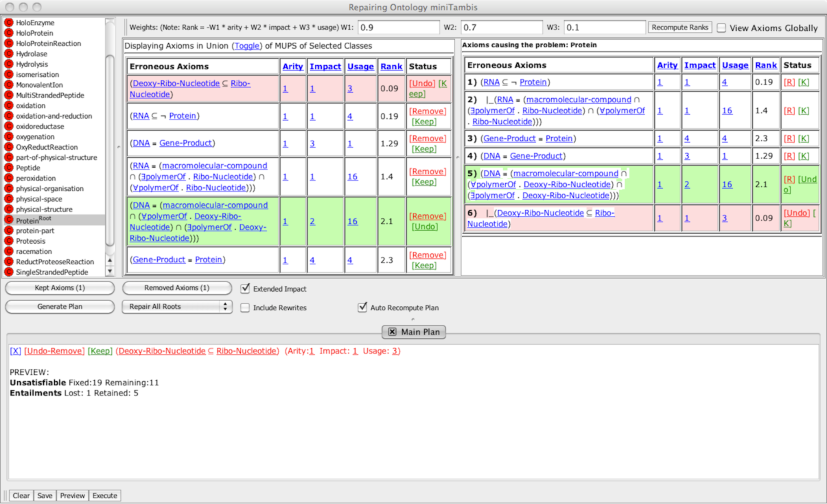
\includegraphics[scale=1]{img/swoop.pdf}
	\caption{A screenshot of the \emph{Repair} tool in \swoop.}
	\label{fig:swoop-screenshot}
}
\end{figure}

Kalyanpur et al.\ \cite{kalyanpur06bh} approached the problem of finding a suitable repair for unsatisfiable classes by introducing a \emph{ranking} on the axioms in justifications. Axioms are ranked according to their frequency, their impact, manually specified test cases by a user (which is an extension to the default impact in order to ensure that specific entailments are preserved), provenance information about the axiom (author, source reliability, time added or modified) and usage of the terms in the axiom signature across the ontology. The repair tool in the \swoop \cite{kalyanpur06sk} editor allows users to specify the weights of the various ranking features, then recommends the preservation or removal of high- or low-ranked axioms, respectively. A screenshot of \swoop's debugging panel is shown in Figure \ref{fig:swoop-screenshot}. While this kind of elaborate debugging support sounds promising, there have not been any in-depth user studies to confirm whether and to which extent ontology developers use the tool and how they benefit from it.

\subsection{Understanding individual justifications}
While the main focus of justification research has been on the performance of justification finding algorithms, in recent years the issue of \emph{understanding} justifications has been receiving increased attention. We know that justifications can significantly reduce user effort by allowing them to focus on a small, \emph{relevant} subset of an ontology; and yet, justifications do not always help all users in understanding the actual \emph{reason} why an entailment holds and in finding a suitable repair.

\subsubsection{Fine-grained justifications}
By definition, a justification is a minimal entailing subset of an ontology; that is, a justification contains axioms as they are \emph{asserted} in the ontology. This means that the axioms in a justification can contain \emph{superfluous} parts, i.e.\ subexpressions on the LHS or RHS of the axiom which do not contribute to the entailment. While such superfluous parts can distract users from the actual cause of an entailment, thus making the justifications more difficult to understand, removing axioms with superfluous parts in the repair process also means a loss of possibly valuable information. 

In order to cope with the issue of superfluity, the notion of \emph{fine-grained} justification was first introduced by Kalyanpur et al.\ \cite{kalyanpur06fj}. This approach was based on the idea of re-writing justification axioms in a normalized form, then splitting the axioms across intersections and only preserving those axioms which are required for the entailment in question to hold. The strategy was implemented in the Swoop editor, using strike-out and colour highlighting to indicate superfluous expressions in axioms---a simple, yet visually effective technique. Lam et al.\ \cite{lam06tk} directly integrated the idea of fine-grained justifications into a repair tool, computing the impact of each axiom rewriting based on the modification of its \emph{subexpressions}.

Based on these first attempts, Horridge et al.\ \cite{horridge08yi} firstly proposed a definition for \emph{laconic} justifications: a laconic justification is a justification which does not contain any superfluous parts, with every subexpression being as \emph{weak} as possible \cite{horridge08yi}. This implies that every subexpression in a laconic justification is relevant to the entailment. The authors \cite{horridge08yi} also describe a method to compute the \emph{preferred} laconic versions of a justification which results in a unique correspondence between a justification and its laconic variants. In short, the process
\begin{compactitem}
\item removes any subexpressions from axioms which are not relevant for the entailment to hold.
\item derives a single subsumption axiom from an equivalence where possible.
\item substitutes class names with the \thing where possible.
\item weakens number restrictions to the smallest number possible.
\end{compactitem}

The following example illustrates several aspects of non-laconicity in a justification:
\begin{examp}
\begin{align*}
\J &=  \{ A \sqsubseteq B ~\conj \leq2 r.C, \exists r.C \sqsubseteq D\} \models A \sqsubseteq D
\end{align*}
\end{examp}
First, we can reduce the intersection in the first axiom to the single expression $\leq2 r.C$ without affecting the entailment. Second, this expression can then be weakened to $\leq1 r.C$. Third, the class name $C$ in both axioms can be substituted with \thing. This results in the laconic justification $\{ A \sqsubseteq \leq1 r.\top, \exists r.\top \sqsubseteq D\}$. 

A survey \cite{horridge11ab} of 72 of OWL ontologies from the NCBO BioPortal\footnote{\url{http://bioportal.bioontology.org/}} revealed that non-laconic justifications are prevalent across OWL ontologies; indeed, the majority of the surveyed ontologies (69 out of 72) contained at least some non-laconic justification for an atomic subsumption, with 29 ontologies containing over 50\% non-laconic justifications. 

\subsubsection{Masking}
Justification \emph{masking} \cite{horridge08yi,horridge10bg} occurs when the actual number of \emph{reasons} why an entailment holds differs from the number of justifications that can be found for the entailment. There exist different types of masking, which are mainly caused by axioms containing superfluous expressions, i.e.\ being non-laconic. The examples given in \cite{horridge10bg} focus on unsatisfiable classes; it can easily be shown, however, that masking also occurs for arbitrary entailments.

\emph{Internal masking} describes a situation where the justification contains more than one reason why an entailment holds, which means that there exist multiple laconic versions of the justification.
\begin{examp}\begin{align*}
\J &=  \{ A \sqsubseteq B \conj C, B \disj C \sqsubseteq D\} \models A \subcls D
\end{align*}\label{ex:internalmasking}\end{examp}
Example \ref{ex:internalmasking} shows a justification \J for \dlax{A \subcls D} which contains two reasons for the entailment. The laconic versions of \J are:
\begin{align*}\J_{1} &=  \{ A \sqsubseteq B, B \sqsubseteq D\}\\
\J_{2} &=  \{ A \sqsubseteq C, C \sqsubseteq D\}\end{align*}

\emph{External masking} involves other axioms from the ontology which do \emph{not} occur in any justifications for an entailment. 
\begin{examp}\begin{align*}
\O &=  \{ A \sqsubseteq C \conj  D, C  \sqsubseteq D\} \entails A \sqsubseteq D
\end{align*}\label{ex:externalmasking}\end{examp}
In the ontology shown in Example \ref{ex:externalmasking} there exists only one justification for the entailment \dlax{A \subcls D}, namely the first axiom \dlax{A \subcls B \conj C}. It is clear to see, however, that the two axioms in \O combined result in another reason for the entailment---but the justification comprising both axioms would violate the minimality condition for justifications.

\emph{Cross masking} is similar to external masking with the difference that the axioms involved are from other \emph{justifications} for the same entailment rather than non-justification axioms.
\begin{examp}\begin{align*}
\J_{1} &=  \{ A \sqsubseteq C \conj D \}\\ 
\J_{2} &=  \{ A \disj C \sqsubseteq D\}
\end{align*}\label{ex:crossmasking}\end{examp}%
In addition to the two justifications $\J_{1}$ and $\J_{2}$ for the entailment $A \sqsubseteq D$, there exists a third reason why the entailment holds, which comprises parts of both justifications: $ \{ A \subcls C, C \subcls D\} \entails A \subcls D$. Again, this third reason,  comprising both axioms, cannot be a justification, as it is non-minimal.

\emph{Shared cores masking} occurs when two \emph{different} justifications have the same reason why an entailment holds, i.e.\ they only differ in their superfluous parts. This implies that the actual number of explanations for an entailment is \emph{lower} than it appears.
\begin{examp}\begin{align*}
\J_{1} &=  \{ A \sqsubseteq D\}\\ 
\J_{2} &=  \{ A \sqsubseteq D \conj \exists r.C\}
\end{align*}\end{examp}
An ontology which contains the two axioms in $\J_{1}$ and $\J_{2}$ has two distinct justifications for the entailment $A \sqsubseteq B$. However, the actual reasons why the entailment holds are identical, as the laconic version of $J_{2}$ is identical to $J_{1}$. 

Masking may cause problems for users attempting to understand or repair an entailment. When repairing a justification where internal, external, or cross masking occurs, a user might only notice and modify one of the reasons, expecting the entailment to no longer hold after the modification. That modification, however, may lead to \emph{another} justification for the entailment---an effect which may be rather surprising. Worse even, the justification may interact with several other axioms to create multiple justifications, a situation which has been found to occur in the NCI thesaurus \cite{horridge11ab}. Furthermore, when analysing justifications for the purpose of gathering ontology metrics, justification masking may lead to over- or under-counting the number of \emph{actual} justifications in an ontology.

It is clear to see that ontology debugging tools need to support users in cases where masking occurs through non-laconicity. Dealing with superfluity in an explanation tool, however, makes it necessary to balance two opposing requirements: first, we want the user to be presented with the most concise explanation as to why an entailment holds, and avoid cluttering and distraction caused by superfluous parts. Second, in order to facilitate understanding and repair, the explanations should directly relate to the asserted axioms in the ontology. To date, there have been no successful approaches to OWL ontology debugging that meet both requirements.
 
 
\subsubsection{Justification-based proofs}
\label{sec:justproofs}
In addition to superfluity, there exist other reasons why a justification can be difficult to understand. Justifications may contain structural patterns and constructors whose implications are unfamiliar or non-obvious to the user. A popular example from the \emph{Movie} ontology illustrates how even a very small justification can be hard to impossible to understand for OWL experts \cite{horridge09zp,horridge10gs}: 
\begin{examp}\begin{align*}
		\J = \{ &\ax{Person \sqsubseteq \neg Movie},\\
		&\ax{RRated \sqsubseteq CatMovie},\\
		&\ax{CatMovie \sqsubseteq Movie},\\
    	&\ax{RRated \eqcls \exists hasScript.ThrillerScript \disj \forall hasViolenceLevel.High},\\
    	&\ax{domain(hasViolenceLevel, Movie)} \} \entails \ax{Person \subcls \nothing}
	\end{align*}\label{ex:movie}\end{examp}
Example \ref{ex:movie} shows a justification for the unsatisfiability of the class \cn{Person} in the \emph{Movie} ontology. Axioms 2 to 5 in the justification entail that \ax{Movie \eqcls \thing}, which implies that \ax{Person \subcls Movie}, which, in turn, contradicts the first axiom that states the disjointness of the classes \cn{Person} and \cn{Movie}. When presented with this justification, subjects tend to give up or question the correctness of the justification \cite{horridge10gs}.

\emph{Justification-based proofs} seek to address the problem of understanding such justifications by providing users with a more detailed explanation which includes not only the justification axioms, but also intermediate entailments such as \ax{Movie \eqcls \thing} in the previous example. Such intermediate entailments, arising from subsets of a justification \J are known as \emph{lemmas}.

In a similar approach to justification-based proofs, Nguyen et al.\ \cite{nguyen12aa} generate natural language proofs based on justifications by identifying frequent sub-patterns, or \emph{rules}, in justifications which lead to such intermediate entailments, then translating the proof trees into natural language. They extracted patterns, restricted to laconic axioms and a maximum size of 4 axioms, from 500 OWL ontologies and identified the 57 most frequent patterns, which are then used as the basis for natural language proofs.


\subsubsection{Cognitive complexity}

To date, there have only been few attempts at investigating the understandability of justifications for OWL users. While there exists a number of user studies to evaluate OWL debugging tools \cite{kalyanpur05mi,lam07aa}, they focus on measuring the time and success rates of the debugging tools and do not offer any further insights into how users interact with the explanations. The first major study on the cognitive complexity of justifications was carried out by Horridge et al.\ \cite{horridge11gj} for the purpose of evaluating a complexity model for justifications which was constructed based on an initial exploratory study \cite{horridge11si}. The study involved 14 students from an MSc class who were presented with a set of items consisting of a set of axioms and an entailment, and were asked to answer whether the entailment followed logically from the axiom set or not. It was found that the complexity predicted by the model coincided partially with the error rate in this task, with some anomalies in the error rates caused by a) superfluity in a justification which the model did not account for, and 2) by a \enquote{flaw} in the experiment protocol which meant test subjects could answer the question correctly, but (presumably) for the wrong reason.

Building on their work on justification-based proofs, Nguyen et al.\ \cite{nguyen12ab}  present an investigation of the difficulty users have with understanding various sub-patterns that occur in OWL justifications. The authors conducted a study on a \enquote{mechanical turk} like web platform where test subjects were presented with natural language reasoning problem which was directly based on one of the 51 (out of 57 identified) justification sub-patterns. Each problem was answered by around 50 people, with correct answers ranging from 100\% for the easiest rule to only 2\% for the most difficult one. While natural language based explanation is potentially highly effective for OWL novices, the resulting proofs are often very large and might be difficult to navigate and understand themselves. 


\subsection{Understanding multiple justifications}

In many ontologies used in practice, we find that there exist multiple justifications for a single entailment. While the possible number of justifications per entailment is exponential in the number of axioms in the ontology \cite{baader07xp}, the average number of justifications found in OWL ontologies is comparatively small \cite{bail11jm}. However, even for justification counts way below the exponential threshold, we are often faced with several dozen to several hundred justifications for a single entailment. When attempting to repair an ontology, such numbers are clearly not suitable for manual repair by a user; and even with a justification-based repair tool which displays all justifications as a list, there is hardly any chance of producing a minimal repair.

Ji et al.\ \cite{ji08en} propose a strategy for reducing the number of justifications a user is confronted with by only computing justifications that are the most \emph{relevant} for an entailment. The approach, which was implemented as part of a plugin to the NeOn Toolkit\footnote{\url{http://www.neon-toolkit.org/}} ontology editor, introduces a selection function based on the amount of signature a justification shares with the entailment. While this relevance-based approach may be helpful when users require only a few justifications for \emph{understanding} an entailment, it does not solve the problem of helping a user repair \emph{all} justifications to break an unwanted entailment.

\subsubsection{Root and derived justifications}
\label{sec:rootderived}

\emph{Root and derived} justifications provide an additional form of explanation support which aims to assist users in the simultaneous repair of multiple entailments. The idea of unsatisfiable classes depending on the unsatisfiability of another class was originally mentioned in \cite{schlobach05tf} and explicitly introduced as root and derived unsatisfiable classes \cite{kalyanpur05mi}. While the initial focus was on entailed unsatisfiable classes, the concept can be easily extended to arbitrary entailments, as shown in \cite{meyer10vd}: given a set of entailments \entset and their justifications \justs, a \emph{derived} justification $\J_{D} \models \eta_{D}$ is a justification which is a superset of some other justification $\J, \eta$. Repairing \J first (e.g.\ by removing or modifying an axiom) will also repair $\J_{D}$. Note that there may be additional reasons for $\eta_{D}$ to hold, which are not covered by this process. A \emph{root} justification is a justification $\J_{R}$ in \justs which is not a superset of any other justification in \justs.

\begin{defn}[Root and derived justifications]
Let \entset be a set of entailments of interest, and \just a justification for an entailment \ent in \entset. \just is called a \emph{root} justification if there exists no justification $\just'$ for an entailment in \entset such that $\just' \subset \just$, else, \just is called a \emph{derived} justification.
\end{defn}

Kalyanpur et al.\ \cite{kalyanpur05mi} carried out the first user study for explanation support in OWL, evaluating the debugging facilities of the ontology editor Swoop. The 12 study subjects were randomly divided into four groups and were given the task to repair unsatisfiable classes in three OWL ontologies using one of three types of debugging tools (clash information from the reasoner and sets of support, root and derived unsatisfiable classes, both), with the fourth group receiving no debugging support at all. Perhaps unsurprisingly, the study found that the group using both the clash information, sets of support (i.e.\ justifications) and root and derived information performed best (i.e.\ fastest) in this task.



\section{Alternative approaches to debugging}
Besides justifications (and approaches closely related to the concept of justifications), there exists a number of alternative approaches to ontology debugging. While these may not be as prevalent as justifications in OWL ontology tools, they represent some relevant solutions to the problem of understanding and debugging formal ontologies, such as proofs, natural language techniques, and semi-automated debugging strategies. Under this label, we also gather other approaches to visualising and understanding ontologies, which, while not explicitly tailored towards debugging, may be helpful tools for understanding and repairing entailments.

\subsection{Proofs}

Formal proofs are considered to be the most prevalent alternative form of explanation for logic-based knowledge bases. One of the first approaches to explaining entailments in the CLASSIC system using proof-like structures was presented by McGuinness and Borgida \cite{mcguinness95jb}. The system omits \enquote{obvious} intermediate steps and provides further filtering strategies in order to generate short and simple explanations. Borgida et al.\ \cite{borgida99cn} first introduced a proof-based explanation system for knowledge bases in the Description Logic \dl{ALC}. The system generates sequent calculus \cite{83aa} style proofs using an extension of a tableaux reasoning algorithm, which are then enriched to create natural language explanations. Aiming to \enquote{provide the simplest explanation possible}, the authors also introduce a \emph{relevance} function which simplifies the proofs by omitting \enquote{irrelevant} parts. The consensus of these proof-based approaches seems to be that good proofs ought to be \enquote{as simple and short as possible}, yet, there have been no formal investigations into how ontology developers interact with such proof-based explanations. 

While proof presentation in other logics has been well studied (e.g.\ \cite{felty1988aa}), surprisingly few authors are concerned with the cognitive aspects of proof understanding. There exist formal definitions of \emph{obvious proof steps} \cite{davis81sz, rudnicki87om}, however, these are merely formulated with the goal of creating \emph{short} proofs and do not investigate other sources of complexity for human readers. By comparison, Lingenfelder \cite{lingenfelder89rm} also considers the skill level of the proof reader to be crucial in order to determine what can be considered \enquote{trivial} in a proof, and emphasises the need for a \emph{user model} in order to provide suitable proofs. 

\subsection{Ontology revision}

Ontology revision as described by Nikitina et al.\ \cite{nikitina12aa} follows a semi-automated approach to ontology repair, with a focus on factually incorrect statements rather than logical errors. In the ontology revision process, a domain experts inspects the set of ontology axioms, then decides whether the axiom is correct (should be accepted) or incorrect (axiom is rejected). Each decision thereby has consequences for other axioms, as they can be either automatically accepted (if they follow logically from the accepted axioms) or rejected (if they violate the already accepted axioms). 

The ontology revision system determines the impact a decision has on the remainder of the axioms (using a ranking function), and presents high impact items first in order to minimize the number of decisions a user has to make. Conceptually, this approach is straightforward and easily understandable for a user, as the cognitive effort is reduced to a simple yes/no decision, and the tool attempts to minimize the number of decisions that need to be made. In order to debug unwanted entailments, e.g.\ unsatisfiable classes, the set of unwanted consequences can be initialised with those erroneous axioms. The accept/decline decisions are then made in order to remove those axioms which lead to the unwanted entailments. 

\subsection{Direct computation of diagnoses}

The direct diagnoses computation approach \cite{friedrich05rg,du08eo,shchekotykhin12aa,rodler12aa} is directly related to justifications, but rather than computing the set of justifications for an entailments which is then repaired by repairing or modifying a minimal hitting set of those justifications, the diagnoses (i.e.\ minimal hitting sets) are computed directly. The direct computation of diagnoses using the hitting set tree algorithm was first proposed by Friedrich and Shchekotykhin \cite{friedrich05rg}. The authors argue that debugging large numbers of conflicts and potentially diagnoses by computing justifications poses a computational challenge, while direct computation of diagnoses provides a more efficient solution. 

Both the ontology revision approach by Nikitina et al.\ and the direct computation of diagnoses show some advantages over computing justifications in terms of computational performance. However, the semi-automated repair presented in \cite{nikitina12aa} means that the user has no direct control over which axioms to remove or modify in order to repair the unwanted entailments, while the direct computation of diagnoses aims exclusively at finding a minimal repair, regardless of the factual correctness or incorrectness of the axioms involved in the diagnoses. Furthermore, neither of the approaches supports \emph{understanding} why those entailments hold, as the users are not presented with the actual \emph{reasons}, but only see a sequence of axioms or a set of diagnoses, respectively. While both approaches aim to reduce the total number of steps taken in the debugging process, they might still require a user to go through a long and tedious revision process when repairing a large number of errors.

\subsection{OntoClean}

OntoClean \cite{guarino02aa,guarino04aa} provides a framework for making modelling decisions in the ontology development process, with a strong focus on correct subumption relationships. This is motivated by a misuse of subsumptions to express other relations than is-a relationships, for example part/whole relationships. OntoClean helps users to validate taxonomies by identifying \emph{metaproperties} of each class, such as \emph{rigidity}, \emph{identity}, \emph{unity}, and \emph{dependency}. The framework then specifies constraints on subsumptions between classes with different properties, such as if a class \dlcn{A} is anti-rigid, i.e.\ an instance of \dlcn{A} can \emph{cease} to be a member of the class, then every subclass of \dlcn{A} must also be anti-rigid. By applying OntoClean guidelines when building taxonomies, ontology developers can prevent subsumption relationships which may later lead to modelling inconsistencies.

\subsection{Ontology comprehension}

Ontology users often require support in understanding an ontology, or parts of it, for example, when integrating an existing ontology into a project, which requires the ontology developer to familiarise themselves with the structure of the adopted ontology. While not specifically aimed at ontology debugging, such comprehension and visualisation tools can  help users to get a better grasp of the relationships between entities in an ontology, which may provide support in the debugging process.

Ontology visualisation tools, such as the OWLViz plugin\footnote{\url{http://www.co-ode.org/downloads/owlviz/}} in \protege, the CropCircles tool \cite{wang06wr} and the, admittedly rather exotic, music score notation of Barzdins and Barinskis \cite{barinskis07uz}, offer ontology users support when exploring an ontology in order to gain an overview of the relationships between its classes.

Visualisation techniques can also be used for the purpose of \emph{model exploration} \cite{bauer09ru}, which can user support in understanding \emph{non-entailment}. Users may want to understand, for instance, why a class is not entailed to be subclass of some other---a fact that cannot be explained by justifications, as it is not possible to point out a particular subset of the ontology that does \emph{not} entail something. The idea underlying model exploration is that seeing (subsets of) the models of an ontology helps users understand the relations between its classes, which, in turn, may support them in understanding why an entailment holds or does \emph{not} hold in the ontology.


\section{Summary and conclusions}
In this chapter, we have laid out the foundations for the work presented in this thesis. We introduced the basic concepts of description logic knowledge bases, such as their syntax, semantics, and standard reasoning services, and introduced the Web Ontology Language OWL. We discussed the scope of logical and non-logical errors which can occur in OWL ontologies and introduced justifications as the currently dominant form of debugging support for entailments of OWL ontologies. This was followed by a closer look at the strategies for computing justifications, as well as some of the applications of justifications for repairing errors in OWL ontologies. Finally, we gave an overview over debugging strategies for description logic knowledge bases which are not directly related to justifications or only make indirect use of them, finding that the majority of approaches do not consider cognitive aspects of how users interact with explanation.

While multiple justifications for entailments of OWL ontologies have been acknowledged as a phenomenon to be found in OWL ontologies, the main focus of research thus far has been the efficiency of computing multiple justifications. In contrast, the issue of how users can find a suitable repair once those justifications have been computed has been largely neglected. There exist some approaches to making individual justifications easier to understand, such as laconic justifications and justification-based proofs, but the specific problem of debugging and repair in the presence of multiple justifications has not been addressed in prior research, except for some work looking at root and derived unsatisfiable classes. Root and derived unsatisfiable classes provide a first level of additional support for a particular relationship between multiple justifications for multiple entailments; yet, there have been no investigations into whether root/derived relationships are indeed a common feature of OWL justifications, what steps can be taken when this feature is not present, and how users can cope with multiple justifications for \emph{single} entailments. Besides, while root and derived unsatisfiable classes indicate that there exist structural relationships between justifications, there have not been any investigations into other such relationships and whether they can be exploited for debugging.

In summary, there does not seem to be a good understanding of how prevalent multiple justifications are in ontologies used in practice, neither are there sophisticated enough coping strategies to help ontology engineers deal with multiple justifications efficiently. These insights motivate the research presented in this thesis, as there is an obvious need for further investigation of the occurrence of multiple justifications, the relations between them, and techniques for reducing both mechanical (the number of steps taken to achieve a goal) as well as mental (the cognitive complexity of the information presented to a user) user effort in the presence of multiple justifications.